










\subsection{Earth-Sun system}








\subsubsection{Stability}

\begin{figure}[H]
    \centering
    \begin{subfigure}{0.5\textwidth}
        \centering
        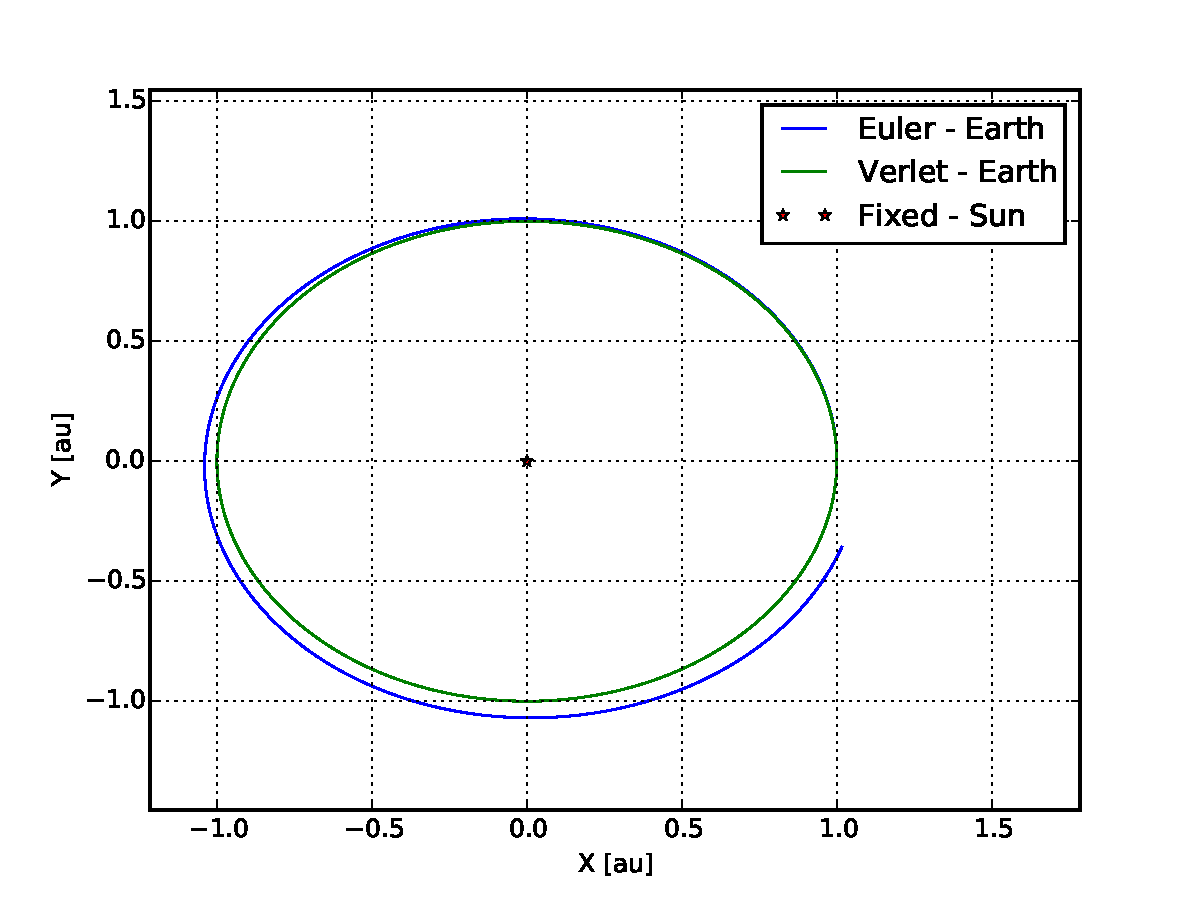
\includegraphics[width=\linewidth]{result/bilder/earth-sun.pdf}
    	\caption{}
    \end{subfigure}%
    ~ 
    \begin{subfigure}{0.5\textwidth}
        \centering
        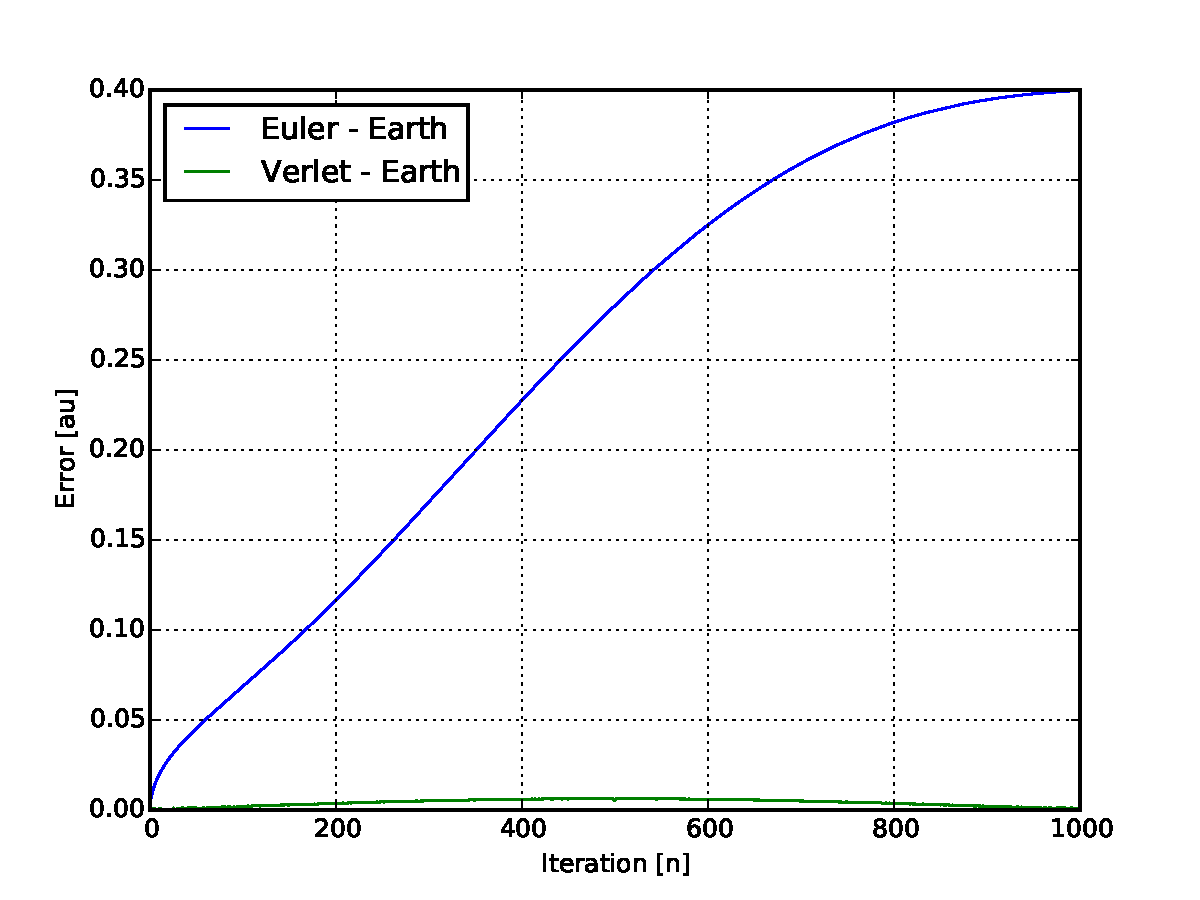
\includegraphics[width=\linewidth]{result/bilder/earth-sun-error.pdf}
        \caption{}
    \end{subfigure}
    \caption{a) shows the orbit of earth around the sun. The intial velocity is set to $2\pi$ in y direction and the start position to 1 au in x direction. b) shows how the error develops. The intial values should give a perfect circular motion. So the error is calculated by $r_i - r_{0}$. It is apparent that the Verlet-Velocity method is a better approximation. This simulation was with 1000 points with the end time of 1 year. Both simulations was produced by \href{https://github.com/erikfsk/Project-3/tree/master/Project3/earth-sun-standard-results}{\textcolor{blue}{plot\_earth\_sun.py}}}
    \label{fig:earth-sun}
\end{figure}


\begin{center}
\label{table:euler-verlet-time}
\captionof{table}{Time table for the different algorithms. The algorithms use nearly the same time. This is not a shocker since the number of FLOPs for the algorithms are similar, see section (\ref{sec:flops}). Note: this is only the result from one test, but several was done. Both algorithms were very close and it seems to be random which is fastest.
\\}
\begin{tabularx}{\textwidth}{c c c c c c c c}
    \hline 
    \hline 
    n & Forward-Euler & Verlet-Velocity &  fastest &&&& $\frac{slowest}{fastest}$\\ 
    \hline
    10 & 0.000136 & 0.000148 & Euler &&&&   1.08823529412   \\ 
    100 & 0.000208 & 0.000179 & Verlet &&&&   1.16201117318   \\ 
    1000 & 0.000392 & 0.000389 & Verlet &&&&  1.00771208226   \\ 
    10000 & 0.002427 & 0.002426 & Verlet &&&&   1.00041220115  \\ 
    100000 & 0.022931 & 0.022293 & Verlet &&&&   1.02861884897   \\ 
    1000000 & 0.167022 & 0.175944 & Euler &&&&   1.05341811258  \\ 
    10000000 & 1.58721 & 1.52666 & Verlet &&&&   1.03966174525  \\ 
    100000000 & 15.1786 & 15.1176 & Verlet &&&&   1.00403503202  \\ 
    \hline
\end{tabularx}
\end{center}
